\chapter{Optimizing the CNN}\label{make}

\section{Processing the images}
For the following steps a simulated dataset containing roughly \num{2000000} gamma events and \num{400000} hadron events has been used.
Every recorded event holds the count of every arrived photon for all \num{1440} pixels for \num{100} consecutive time frames of \num{5}\,\si{\nano\second}.
To reduce these \num{144000} variables all photons have been summed along the time axis for every pixel separately (time series summation).

\begin{figure}
    \centering
    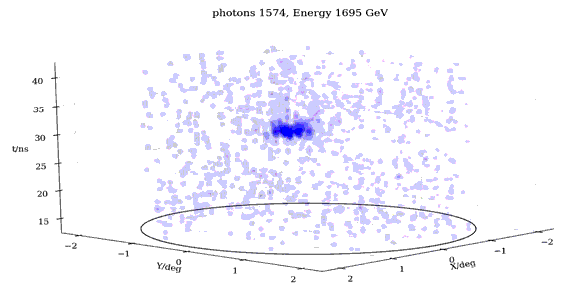
\includegraphics[width=8cm]{Plots/Photon_Event_3D.png}
    \caption{Structure of an example event}
    \label{fig:example_event}
\end{figure}

Naturally many photons not derived from the Cherenkov light are contained in the image.
Since the telescope triggers all events approximately at the same time frame
the event itself can be cut out by removing preceding and succeeding time frames filled with distracting noise.
This results in cleaner denoised images for the pattern detection in the CNN.

\begin{figure}
    \centering
    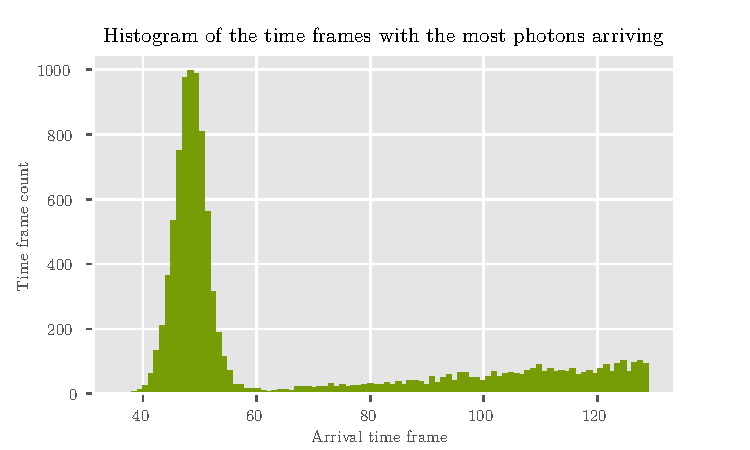
\includegraphics[scale=1]{Plots/Arrivaltimes.pdf}
    \caption{The brightest time frames of \num{10000} events are shown in the histogram. Almost all frames cluster around a specific triggering time. By cutting out and using only this cluster noise can be reduced.}
    \label{fig:arrivaltimes}
\end{figure}

For \num{10000} events the time frame with the most photons arriving has been computed.
These bright time frames should most likely contain the events to examine.
By creating a histogram of these time frames it highlights
that the telescope triggers the events nearly every time between the frames \num{35} and \num{60}.
As a result only this range of frames will be used for the denoised images, dropping all other frames containing mostly noise.

In the following paragraph all architectures will be evaluated on the flat greyscale images
containing all photons as well as the denoised ones.


\section{Comparing the architectures}
At this step every tested network architecture is composed of convolution layers (c)
followed by a pooling layer and fully connected layers (f).
The architecture notation follows this example:

\begin{itemize}
\item A '3c\_2f' architecture translates to a network
starting with three convolution and pooling layers and ending with two fully connected layers.
\end{itemize}

There are four important hyperparameters for this kind of networks:

\begin{itemize}
\item The number of images in one batch fed to the network (batch-size)
\item The size of the patch/kernel in the convolution layer (patch-size)
\item The number of feature maps the convolution layer computes (depth)
\item The number of hidden nodes contained in the fully connected layers (hidden-nodes)
\end{itemize}

For all parameter a random grid search was performed in the course of the following steps.
To dismiss random fluctuation in the networks performance caused among others by the grid search
\num{50} networks have been trained for every architecture.

The common proceeding of using a separate training, validation and testing dataset has been adapted.
To measure the network's performance the area under the curve score (AUC) is used.
The training of a network is terminated when the AUC-score of the validation dataset does not rise anymore (early stopping).

\begin{figure}
\centering
\begin{subfigure}{.5\textwidth}
  \centering
  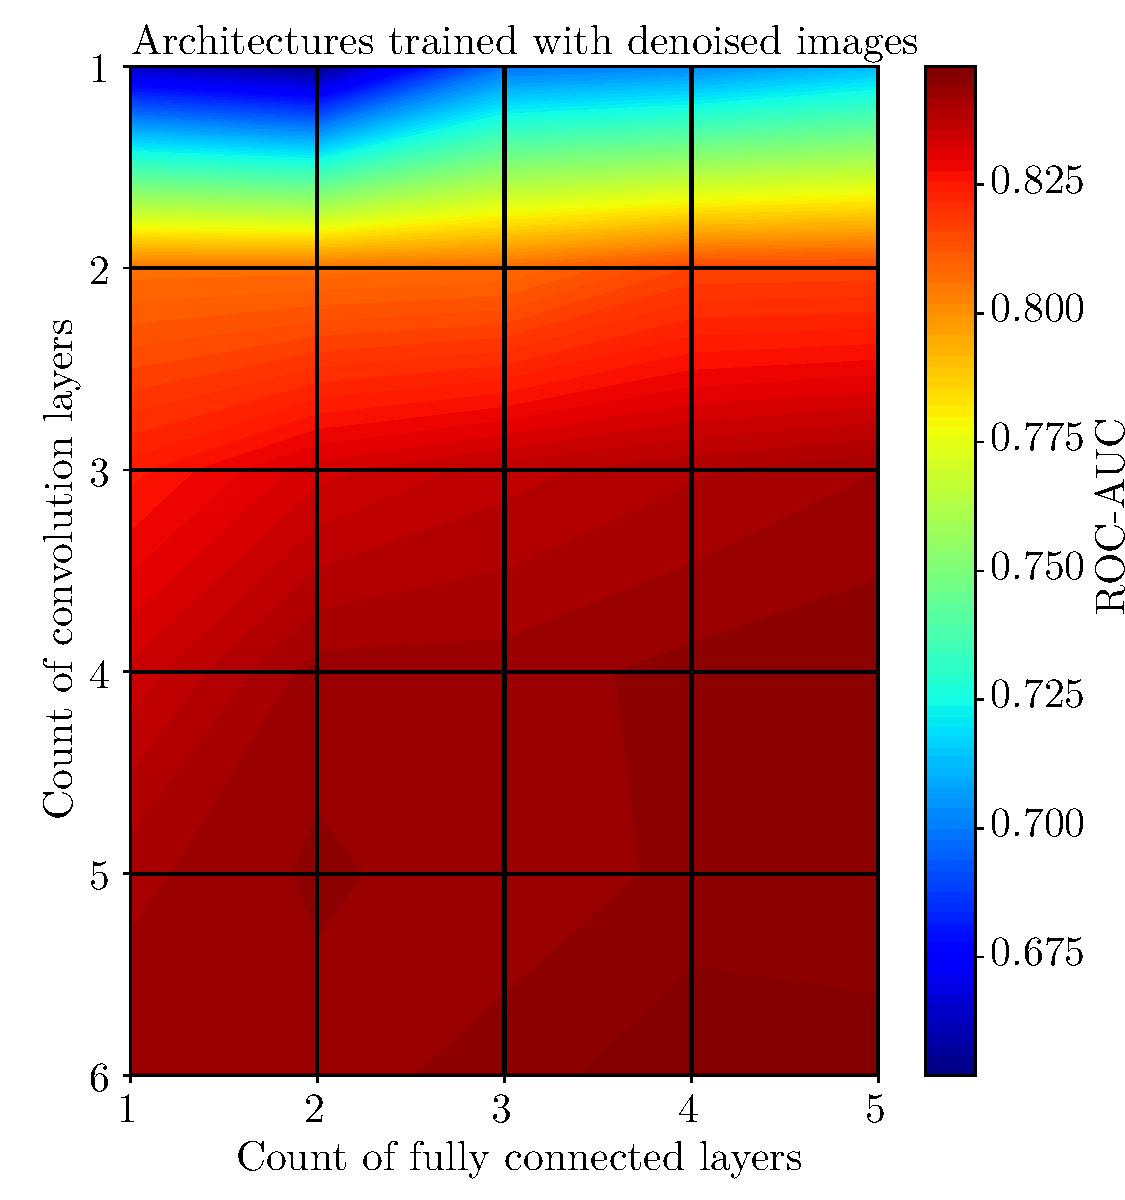
\includegraphics[scale=0.35]{Plots/Architectures_AUC_denoised.pdf}
  \caption{CNNs on denoised images}
  \label{fig:heatmap_denoised}
\end{subfigure}%
\begin{subfigure}{.5\textwidth}
  \centering
  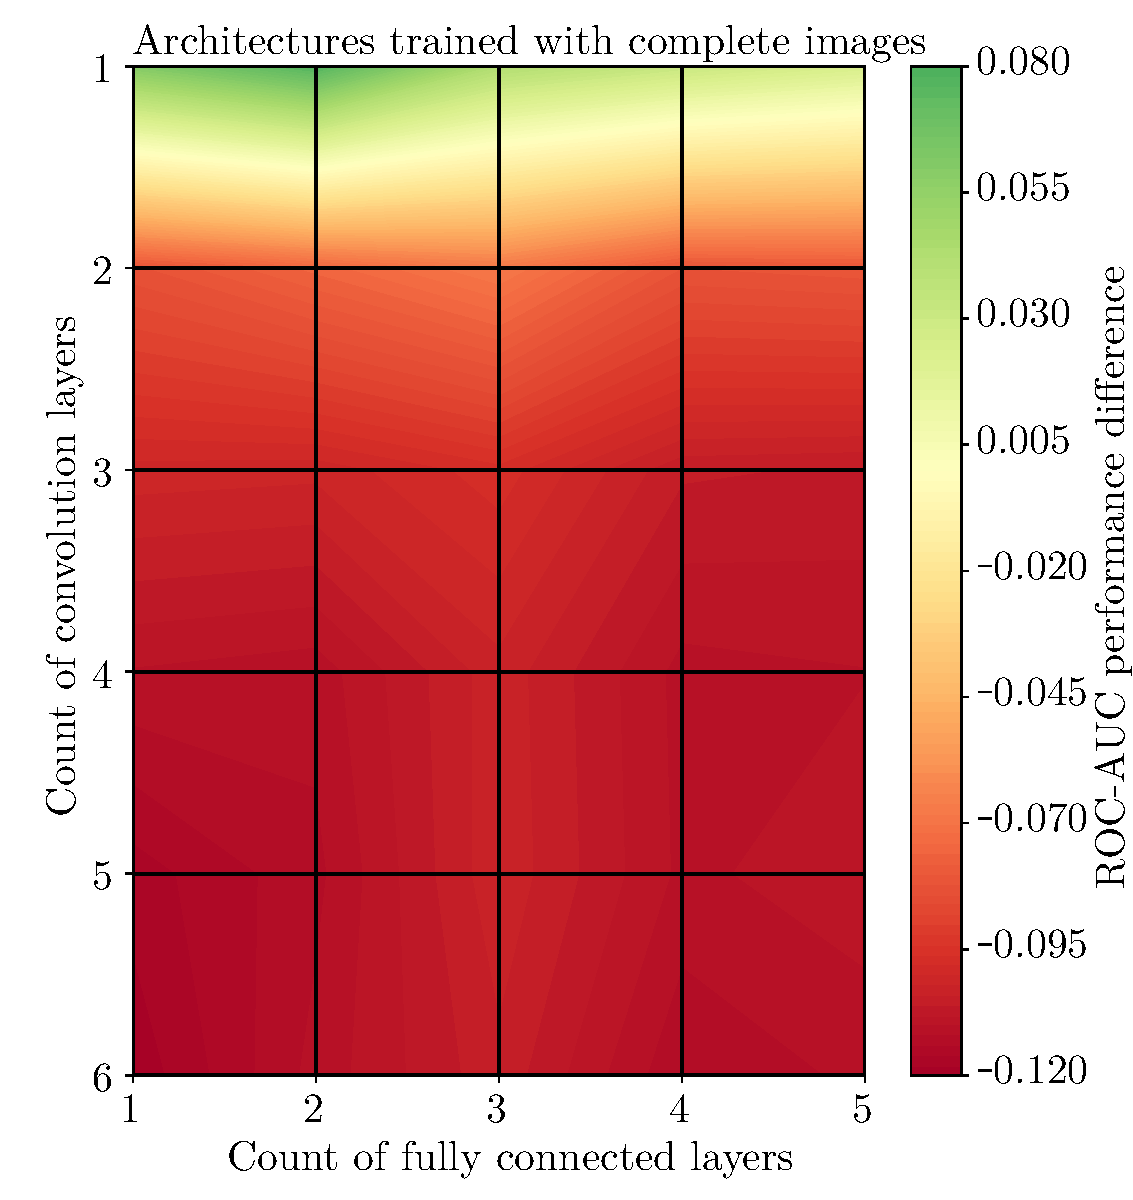
\includegraphics[scale=0.35]{Plots/Architectures_AUC_noised.pdf}
  \caption{CNNs on noisy images}
  \label{fig:heatmap_noised}
\end{subfigure}
\caption{The AUC performances of \num{30} architectures are beeing compared on both denoised and noisy images. Since denoised images perform better the second plot shows the AUC's difference to the better performing one.}
\label{fig:heatmaps}
\end{figure}

By comparing the networks trained on noisy and denoised images it becomes apparent
that denoised images evoke a much more reliable and therefore better network.
Only in the bad performing shallow networks they are inferior to noisy images.

Looking at the architectures it appears that unambiguously deeper networks perform much better than shallow ones.
The number of feature generating convolution layers seems to have a greater impact on the AUC score
compared to the number of fully connected layers.

\begin{figure}
    \centering
    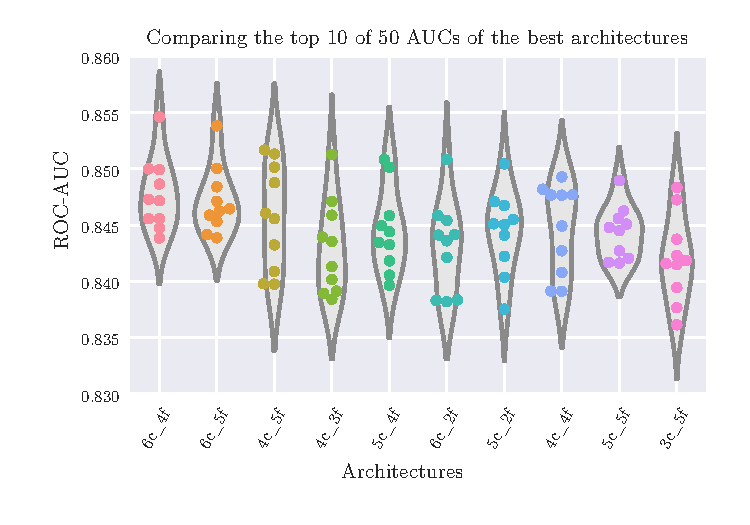
\includegraphics[scale=1]{Plots/Best_denoised_architectures.pdf}
    \caption{For the comparison of the best \num{10} denoised architectures the \num{10} best performing networks of \num{50} trained ones are beeing shown in this plot.}
    \label{fig:top_cnn_architectures}
\end{figure}

By examining the best performing denoised deep network architectures it shows
that only gradually differences separate the best networks from each other.
Since a sample of only \num{50} trained networks guarantees no statistical certainty
no distinct best architecture can be proclaimed.

It can be stated that deeper networks perform better on the given task
and the more generated features the higher the AUC score.
Additionally using only the important part of the recorded events
and dropping some noise increases the network's performance as well.

For a meaningful statement concerning the architectures the hyperparameters of the networks will be investigated.
Since the optimal values for the hyperparameters could not be determined beforehand the training
all parameters for the above researches were randomly chosen from a suitable value range.
Therefore a statement can be issued afterwards to narrow this range down or investigate a more promising value range.




\section{Regularizing the network}
The best performing '3c\_3f' architecture is settled for further investigations to reduce the feature space to explore.
To ensure a stable behavior of the network regularizing dropout layers will be integrated into the network's architecture.
Since the layer can be combined with every existing layer in the network
and likewise can adopt different values for the amount of data to drop out in every layer
a large feature space as to be evaluated.
As adding dropout to a network extends the training time many times over only a few positions can be tested.

\begin{figure}
    \centering
    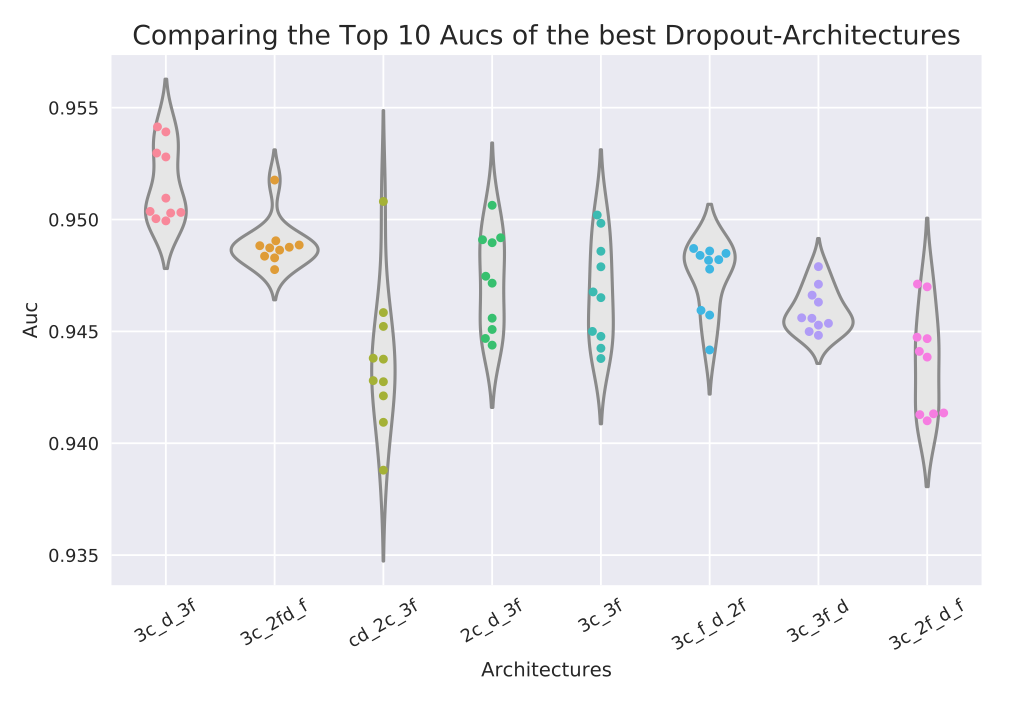
\includegraphics[width=10cm]{Plots/Randomized_Dropout_Model_Comparison.png}
    \caption{Comparing AUCs of different Dropout positions in the CNNs}
    \label{fig:random_dropout}
\end{figure}

Positioning the dropout layer right between the convolution layers and the following fully connected layers
appears to have the most positive impact on the networks performance.
Regularizing the fully connected layers seems to strengthen the network as well.
On the contrary dropping to much information in the convolution layers weakens the network over all.
Therefore the dropout rate is the most important factor rather than the layers position.

It is registered to use dropout layers in every layer, but using different dropout rates.
The following rates were taken from corresponding literature.

\begin{table}
    \centering
    \caption{Choosing the drpooutrates for the different dropout positions}
    \label{tab:dropoutrates}
    \begin{tabular}{S[table-format=4.2] S[table-format=3.2]}
        \toprule
        {Dropout position}  & {dropoutrate} \\
        \midrule
        1 & 0.90 \\
        2 & 0.75 \\
        3 & 0.50 \\
        \bottomrule
    \end{tabular}
\end{table}

Since dropout prolongs the networks training cycle and increases the difficulty to train long networks in general,
pretraining is used to enable efficient training of many layers.

A short network containing dropout layers is trained for a few cycles and the layers adjust their inner values using gradient decent.
Afterwards new layers are appended to the network and the short training cycle starts again.
In this case training cycles consisting of 0k/5k/10k batches are being compared.
To complete the training after the network grew to its full length a normal training cycle with early stopping is added.

\begin{figure}
    \centering
    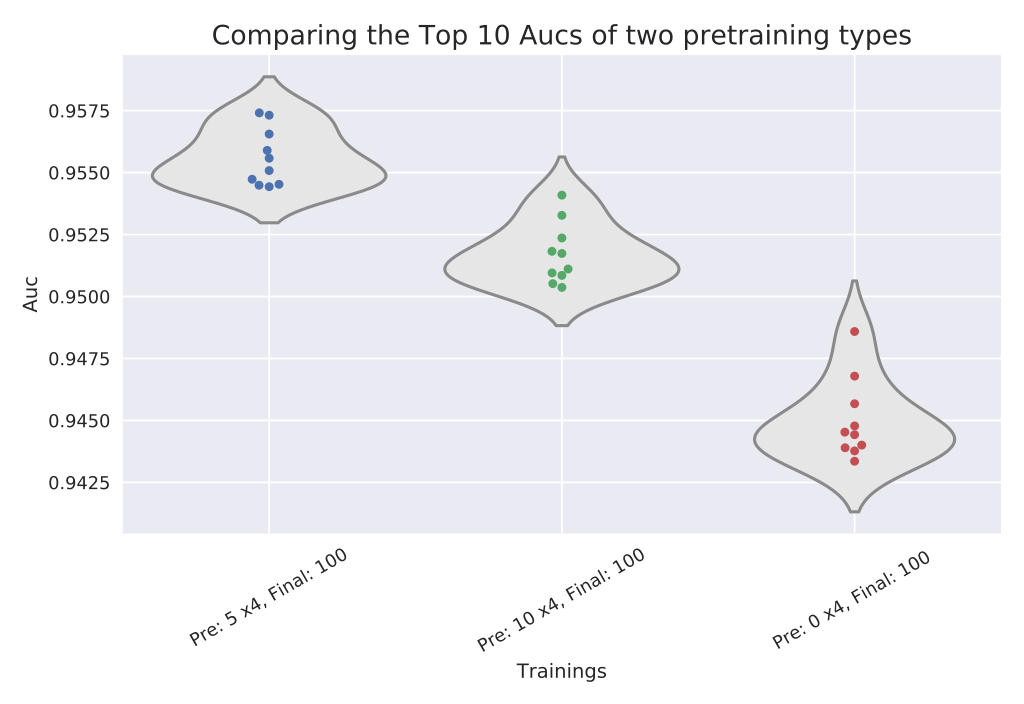
\includegraphics[width=10cm]{Plots/Randomized_Pretraining_Model_Comparison.png}
    \caption{Comparing AUCs of pretrained to normaly trained CNNs}
    \label{fig:random_pretraining}
\end{figure}

Using different amounts of pretraining batches the results emphasize an increase in the performance.
There seems to be a maximum in between using no pretraining at all and using 10k batches for the pretraining of every added layer.
